\documentclass[twoside]{book}

% Packages required by doxygen
\usepackage{fixltx2e}
\usepackage{calc}
\usepackage{doxygen}
\usepackage{graphicx}
\usepackage[utf8]{inputenc}
\usepackage{makeidx}
\usepackage{multicol}
\usepackage{multirow}
\PassOptionsToPackage{warn}{textcomp}
\usepackage{textcomp}
\usepackage[nointegrals]{wasysym}
\usepackage[table]{xcolor}

% Font selection
\usepackage[T1]{fontenc}
\usepackage{mathptmx}
\usepackage[scaled=.90]{helvet}
\usepackage{courier}
\usepackage{amssymb}
\usepackage{sectsty}
\renewcommand{\familydefault}{\sfdefault}
\allsectionsfont{%
  \fontseries{bc}\selectfont%
  \color{darkgray}%
}
\renewcommand{\DoxyLabelFont}{%
  \fontseries{bc}\selectfont%
  \color{darkgray}%
}
\newcommand{\+}{\discretionary{\mbox{\scriptsize$\hookleftarrow$}}{}{}}

% Page & text layout
\usepackage{geometry}
\geometry{%
  a4paper,%
  top=2.5cm,%
  bottom=2.5cm,%
  left=2.5cm,%
  right=2.5cm%
}
\tolerance=750
\hfuzz=15pt
\hbadness=750
\setlength{\emergencystretch}{15pt}
\setlength{\parindent}{0cm}
\setlength{\parskip}{0.2cm}
\makeatletter
\renewcommand{\paragraph}{%
  \@startsection{paragraph}{4}{0ex}{-1.0ex}{1.0ex}{%
    \normalfont\normalsize\bfseries\SS@parafont%
  }%
}
\renewcommand{\subparagraph}{%
  \@startsection{subparagraph}{5}{0ex}{-1.0ex}{1.0ex}{%
    \normalfont\normalsize\bfseries\SS@subparafont%
  }%
}
\makeatother

% Headers & footers
\usepackage{fancyhdr}
\pagestyle{fancyplain}
\fancyhead[LE]{\fancyplain{}{\bfseries\thepage}}
\fancyhead[CE]{\fancyplain{}{}}
\fancyhead[RE]{\fancyplain{}{\bfseries\leftmark}}
\fancyhead[LO]{\fancyplain{}{\bfseries\rightmark}}
\fancyhead[CO]{\fancyplain{}{}}
\fancyhead[RO]{\fancyplain{}{\bfseries\thepage}}
\fancyfoot[LE]{\fancyplain{}{}}
\fancyfoot[CE]{\fancyplain{}{}}
\fancyfoot[RE]{\fancyplain{}{\bfseries\scriptsize Generated on Wed Nov 5 2014 13\+:27\+:40 for Route\+Finder by Doxygen }}
\fancyfoot[LO]{\fancyplain{}{\bfseries\scriptsize Generated on Wed Nov 5 2014 13\+:27\+:40 for Route\+Finder by Doxygen }}
\fancyfoot[CO]{\fancyplain{}{}}
\fancyfoot[RO]{\fancyplain{}{}}
\renewcommand{\footrulewidth}{0.4pt}
\renewcommand{\chaptermark}[1]{%
  \markboth{#1}{}%
}
\renewcommand{\sectionmark}[1]{%
  \markright{\thesection\ #1}%
}

% Indices & bibliography
\usepackage{natbib}
\usepackage[titles]{tocloft}
\setcounter{tocdepth}{3}
\setcounter{secnumdepth}{5}
\makeindex

% Hyperlinks (required, but should be loaded last)
\usepackage{ifpdf}
\ifpdf
  \usepackage[pdftex,pagebackref=true]{hyperref}
\else
  \usepackage[ps2pdf,pagebackref=true]{hyperref}
\fi
\hypersetup{%
  colorlinks=true,%
  linkcolor=blue,%
  citecolor=blue,%
  unicode%
}

% Custom commands
\newcommand{\clearemptydoublepage}{%
  \newpage{\pagestyle{empty}\cleardoublepage}%
}


%===== C O N T E N T S =====

\begin{document}

% Titlepage & ToC
\hypersetup{pageanchor=false,
             bookmarks=true,
             bookmarksnumbered=true,
             pdfencoding=unicode
            }
\pagenumbering{roman}
\begin{titlepage}
\vspace*{7cm}
\begin{center}%
{\Large Route\+Finder }\\
\vspace*{1cm}
{\large Generated by Doxygen 1.8.8}\\
\vspace*{0.5cm}
{\small Wed Nov 5 2014 13:27:40}\\
\end{center}
\end{titlepage}
\clearemptydoublepage
\tableofcontents
\clearemptydoublepage
\pagenumbering{arabic}
\hypersetup{pageanchor=true}

%--- Begin generated contents ---
\chapter{Hierarchical Index}
\section{Class Hierarchy}
This inheritance list is sorted roughly, but not completely, alphabetically\+:\begin{DoxyCompactList}
\item \contentsline{section}{Edge}{\pageref{classEdge}}{}
\item \contentsline{section}{Network}{\pageref{classNetwork}}{}
\item \contentsline{section}{Node}{\pageref{classNode}}{}
\item \contentsline{section}{Route}{\pageref{classRoute}}{}
\item \contentsline{section}{Solver}{\pageref{classSolver}}{}
\begin{DoxyCompactList}
\item \contentsline{section}{Sim\+Annealing\+Alg}{\pageref{classSimAnnealingAlg}}{}
\end{DoxyCompactList}
\end{DoxyCompactList}

\chapter{Class Index}
\section{Class List}
Here are the classes, structs, unions and interfaces with brief descriptions\+:\begin{DoxyCompactList}
\item\contentsline{section}{\hyperlink{classEdge}{Edge} }{\pageref{classEdge}}{}
\item\contentsline{section}{\hyperlink{classNetwork}{Network} }{\pageref{classNetwork}}{}
\item\contentsline{section}{\hyperlink{classNode}{Node} }{\pageref{classNode}}{}
\item\contentsline{section}{\hyperlink{classRoute}{Route} }{\pageref{classRoute}}{}
\item\contentsline{section}{\hyperlink{classSimAnnealingAlg}{Sim\+Annealing\+Alg} }{\pageref{classSimAnnealingAlg}}{}
\item\contentsline{section}{\hyperlink{classSolver}{Solver} }{\pageref{classSolver}}{}
\end{DoxyCompactList}

\chapter{Class Documentation}
\hypertarget{classEdge}{\section{Edge Class Reference}
\label{classEdge}\index{Edge@{Edge}}
}


{\ttfamily \#include $<$Edge.\+h$>$}

\subsection*{Public Member Functions}
\begin{DoxyCompactItemize}
\item 
\hyperlink{classEdge_a8f25ebc010f7bd477335f905643d34bf}{Edge} (unsigned int id, \hyperlink{classNode}{Node} $\ast$start, \hyperlink{classNode}{Node} $\ast$end, const double weight, const Transport\+Type type)
\item 
unsigned int \hyperlink{classEdge_ab14a1f1e26da641effaa7af1e36bd410}{get\+I\+D} () const 
\item 
double \hyperlink{classEdge_ad52d5996050993b96b0b04d68f14f4e4}{get\+Weight} () const 
\item 
const \hyperlink{classNode}{Node} $\ast$ \hyperlink{classEdge_a88540e6c5ab8ad2aa4343a8f21339707}{get\+Start\+Node} () const 
\item 
const \hyperlink{classNode}{Node} $\ast$ \hyperlink{classEdge_abeb6634d35c7c5c1706bc90d91b12c37}{get\+End\+Node} () const 
\item 
Transport\+Type \hyperlink{classEdge_aa38a79bf1da5e02ebd57292c73bfd5fa}{get\+Type} () const 
\item 
void \hyperlink{classEdge_a7ba1bfa5c9c7972d2c31b2c3ba3d7c69}{set\+Weight} (double w)
\item 
void \hyperlink{classEdge_a6fd6d3fd58d73f04b763e2a5bfa6e7e0}{set\+Type} (Transport\+Type t)
\item 
bool \hyperlink{classEdge_a5e15d0508aa070e0dfb9d8b63f1fd510}{operator==} (const \hyperlink{classEdge}{Edge} \&e) const 
\item 
bool \hyperlink{classEdge_a71932326f1787effb05a27254ec354f4}{operator!=} (const \hyperlink{classEdge}{Edge} \&e) const 
\item 
bool \hyperlink{classEdge_a2dd271913eaa0f6250d764170055a3e9}{operator$<$} (const \hyperlink{classEdge}{Edge} \&e) const 
\item 
\hyperlink{classEdge}{Edge} \& \hyperlink{classEdge_ad61a4407d09b063f1d36827cdaa8cfa7}{operator=} (const \hyperlink{classEdge}{Edge} \&e)
\end{DoxyCompactItemize}
\subsection*{Friends}
\begin{DoxyCompactItemize}
\item 
std\+::ostream \& \hyperlink{classEdge_a25f0a91097a6c9b29db3305b469895aa}{operator$<$$<$} (std\+::ostream \&s, const \hyperlink{classEdge}{Edge} \&e)
\end{DoxyCompactItemize}


\subsection{Detailed Description}
Object used for storage of one connections. Includes info about start and end positions, type of connection and weight of it. 

\subsection{Constructor \& Destructor Documentation}
\hypertarget{classEdge_a8f25ebc010f7bd477335f905643d34bf}{\index{Edge@{Edge}!Edge@{Edge}}
\index{Edge@{Edge}!Edge@{Edge}}
\subsubsection[{Edge}]{\setlength{\rightskip}{0pt plus 5cm}Edge\+::\+Edge (
\begin{DoxyParamCaption}
\item[{unsigned int}]{id, }
\item[{{\bf Node} $\ast$}]{start, }
\item[{{\bf Node} $\ast$}]{end, }
\item[{const double}]{weight, }
\item[{const Transport\+Type}]{type}
\end{DoxyParamCaption}
)}}\label{classEdge_a8f25ebc010f7bd477335f905643d34bf}
Constructor of \hyperlink{classEdge}{Edge} object. 
\begin{DoxyParams}{Parameters}
{\em id} & Identificator of object. \\
\hline
{\em start} & Pointer to \hyperlink{classNode}{Node} assigned as starting position. \\
\hline
{\em end} & Pointer to \hyperlink{classNode}{Node} assigned as ending position. \\
\hline
{\em weight} & Given weight. \\
\hline
{\em type} & Enumerated value describing type of route. \\
\hline
\end{DoxyParams}


\subsection{Member Function Documentation}
\hypertarget{classEdge_abeb6634d35c7c5c1706bc90d91b12c37}{\index{Edge@{Edge}!get\+End\+Node@{get\+End\+Node}}
\index{get\+End\+Node@{get\+End\+Node}!Edge@{Edge}}
\subsubsection[{get\+End\+Node}]{\setlength{\rightskip}{0pt plus 5cm}const {\bf Node} $\ast$ Edge\+::get\+End\+Node (
\begin{DoxyParamCaption}
{}
\end{DoxyParamCaption}
) const}}\label{classEdge_abeb6634d35c7c5c1706bc90d91b12c37}
\begin{DoxyReturn}{Returns}
Returns pointer to ending \hyperlink{classNode}{Node}. 
\end{DoxyReturn}
\hypertarget{classEdge_ab14a1f1e26da641effaa7af1e36bd410}{\index{Edge@{Edge}!get\+I\+D@{get\+I\+D}}
\index{get\+I\+D@{get\+I\+D}!Edge@{Edge}}
\subsubsection[{get\+I\+D}]{\setlength{\rightskip}{0pt plus 5cm}unsigned int Edge\+::get\+I\+D (
\begin{DoxyParamCaption}
{}
\end{DoxyParamCaption}
) const}}\label{classEdge_ab14a1f1e26da641effaa7af1e36bd410}
\begin{DoxyReturn}{Returns}
Returns id of itself. 
\end{DoxyReturn}
\hypertarget{classEdge_a88540e6c5ab8ad2aa4343a8f21339707}{\index{Edge@{Edge}!get\+Start\+Node@{get\+Start\+Node}}
\index{get\+Start\+Node@{get\+Start\+Node}!Edge@{Edge}}
\subsubsection[{get\+Start\+Node}]{\setlength{\rightskip}{0pt plus 5cm}const {\bf Node} $\ast$ Edge\+::get\+Start\+Node (
\begin{DoxyParamCaption}
{}
\end{DoxyParamCaption}
) const}}\label{classEdge_a88540e6c5ab8ad2aa4343a8f21339707}
\begin{DoxyReturn}{Returns}
Returns pointer to starting \hyperlink{classNode}{Node}. 
\end{DoxyReturn}
\hypertarget{classEdge_aa38a79bf1da5e02ebd57292c73bfd5fa}{\index{Edge@{Edge}!get\+Type@{get\+Type}}
\index{get\+Type@{get\+Type}!Edge@{Edge}}
\subsubsection[{get\+Type}]{\setlength{\rightskip}{0pt plus 5cm}Transport\+Type Edge\+::get\+Type (
\begin{DoxyParamCaption}
{}
\end{DoxyParamCaption}
) const}}\label{classEdge_aa38a79bf1da5e02ebd57292c73bfd5fa}
\begin{DoxyReturn}{Returns}
Returns Transport\+Type enum value describing type. 
\end{DoxyReturn}
\hypertarget{classEdge_ad52d5996050993b96b0b04d68f14f4e4}{\index{Edge@{Edge}!get\+Weight@{get\+Weight}}
\index{get\+Weight@{get\+Weight}!Edge@{Edge}}
\subsubsection[{get\+Weight}]{\setlength{\rightskip}{0pt plus 5cm}double Edge\+::get\+Weight (
\begin{DoxyParamCaption}
{}
\end{DoxyParamCaption}
) const}}\label{classEdge_ad52d5996050993b96b0b04d68f14f4e4}
\begin{DoxyReturn}{Returns}
Returns weight of itself. 
\end{DoxyReturn}
\hypertarget{classEdge_a71932326f1787effb05a27254ec354f4}{\index{Edge@{Edge}!operator"!=@{operator"!=}}
\index{operator"!=@{operator"!=}!Edge@{Edge}}
\subsubsection[{operator"!=}]{\setlength{\rightskip}{0pt plus 5cm}bool Edge\+::operator!= (
\begin{DoxyParamCaption}
\item[{const {\bf Edge} \&}]{e}
\end{DoxyParamCaption}
) const}}\label{classEdge_a71932326f1787effb05a27254ec354f4}
Compares itself id with given edge id. 
\begin{DoxyParams}{Parameters}
{\em e} & Given \hyperlink{classEdge}{Edge}. \\
\hline
\end{DoxyParams}
\begin{DoxyReturn}{Returns}
True if ids are not equal, false otherwise. 
\end{DoxyReturn}
\hypertarget{classEdge_a2dd271913eaa0f6250d764170055a3e9}{\index{Edge@{Edge}!operator$<$@{operator$<$}}
\index{operator$<$@{operator$<$}!Edge@{Edge}}
\subsubsection[{operator$<$}]{\setlength{\rightskip}{0pt plus 5cm}bool Edge\+::operator$<$ (
\begin{DoxyParamCaption}
\item[{const {\bf Edge} \&}]{e}
\end{DoxyParamCaption}
) const}}\label{classEdge_a2dd271913eaa0f6250d764170055a3e9}
Compares itself id with given edge id. Method used in \hyperlink{classNetwork}{Network} class. 
\begin{DoxyParams}{Parameters}
{\em e} & Given \hyperlink{classEdge}{Edge}. \\
\hline
\end{DoxyParams}
\begin{DoxyReturn}{Returns}
True if this-\/$>$id is smaller than e.\+id, false otherwise. 
\end{DoxyReturn}
\hypertarget{classEdge_ad61a4407d09b063f1d36827cdaa8cfa7}{\index{Edge@{Edge}!operator=@{operator=}}
\index{operator=@{operator=}!Edge@{Edge}}
\subsubsection[{operator=}]{\setlength{\rightskip}{0pt plus 5cm}{\bf Edge} \& Edge\+::operator= (
\begin{DoxyParamCaption}
\item[{const {\bf Edge} \&}]{e}
\end{DoxyParamCaption}
)}}\label{classEdge_ad61a4407d09b063f1d36827cdaa8cfa7}
Assign operator. 
\begin{DoxyParams}{Parameters}
{\em e} & Given \hyperlink{classEdge}{Edge}. \\
\hline
\end{DoxyParams}
\begin{DoxyReturn}{Returns}
Reference to itself. 
\end{DoxyReturn}
\hypertarget{classEdge_a5e15d0508aa070e0dfb9d8b63f1fd510}{\index{Edge@{Edge}!operator==@{operator==}}
\index{operator==@{operator==}!Edge@{Edge}}
\subsubsection[{operator==}]{\setlength{\rightskip}{0pt plus 5cm}bool Edge\+::operator== (
\begin{DoxyParamCaption}
\item[{const {\bf Edge} \&}]{e}
\end{DoxyParamCaption}
) const}}\label{classEdge_a5e15d0508aa070e0dfb9d8b63f1fd510}
Compares itself id with given edge id. 
\begin{DoxyParams}{Parameters}
{\em e} & Given \hyperlink{classEdge}{Edge}. \\
\hline
\end{DoxyParams}
\begin{DoxyReturn}{Returns}
True if ids are equal, false otherwise. 
\end{DoxyReturn}
\hypertarget{classEdge_a6fd6d3fd58d73f04b763e2a5bfa6e7e0}{\index{Edge@{Edge}!set\+Type@{set\+Type}}
\index{set\+Type@{set\+Type}!Edge@{Edge}}
\subsubsection[{set\+Type}]{\setlength{\rightskip}{0pt plus 5cm}void Edge\+::set\+Type (
\begin{DoxyParamCaption}
\item[{Transport\+Type}]{t}
\end{DoxyParamCaption}
)}}\label{classEdge_a6fd6d3fd58d73f04b763e2a5bfa6e7e0}
Sets type to given. 
\begin{DoxyParams}{Parameters}
{\em t} & Given type value. Should be not equal to U\+N\+K\+N\+O\+W\+N. \\
\hline
\end{DoxyParams}
\hypertarget{classEdge_a7ba1bfa5c9c7972d2c31b2c3ba3d7c69}{\index{Edge@{Edge}!set\+Weight@{set\+Weight}}
\index{set\+Weight@{set\+Weight}!Edge@{Edge}}
\subsubsection[{set\+Weight}]{\setlength{\rightskip}{0pt plus 5cm}void Edge\+::set\+Weight (
\begin{DoxyParamCaption}
\item[{double}]{w}
\end{DoxyParamCaption}
)}}\label{classEdge_a7ba1bfa5c9c7972d2c31b2c3ba3d7c69}
Sets weight to given. 
\begin{DoxyParams}{Parameters}
{\em w} & Given weight value. Should be greater than 0. \\
\hline
\end{DoxyParams}


\subsection{Friends And Related Function Documentation}
\hypertarget{classEdge_a25f0a91097a6c9b29db3305b469895aa}{\index{Edge@{Edge}!operator$<$$<$@{operator$<$$<$}}
\index{operator$<$$<$@{operator$<$$<$}!Edge@{Edge}}
\subsubsection[{operator$<$$<$}]{\setlength{\rightskip}{0pt plus 5cm}std\+::ostream\& operator$<$$<$ (
\begin{DoxyParamCaption}
\item[{std\+::ostream \&}]{s, }
\item[{const {\bf Edge} \&}]{e}
\end{DoxyParamCaption}
)\hspace{0.3cm}{\ttfamily [friend]}}}\label{classEdge_a25f0a91097a6c9b29db3305b469895aa}
Operator used for console debug purposes. 
\begin{DoxyParams}{Parameters}
{\em s} & Stream which is used for output. \\
\hline
{\em e} & \hyperlink{classEdge}{Edge} on which operator is called. \\
\hline
\end{DoxyParams}
\begin{DoxyReturn}{Returns}
Given stream. 
\end{DoxyReturn}


The documentation for this class was generated from the following files\+:\begin{DoxyCompactItemize}
\item 
/home/vka/\+Workspace/\+Route\+Finder/src/Edge.\+h\item 
/home/vka/\+Workspace/\+Route\+Finder/src/Edge.\+cpp\end{DoxyCompactItemize}

\hypertarget{classNetwork}{\section{Network Class Reference}
\label{classNetwork}\index{Network@{Network}}
}


{\ttfamily \#include $<$Network.\+h$>$}

\subsection*{Public Member Functions}
\begin{DoxyCompactItemize}
\item 
\hyperlink{classNetwork_a3cc2fb4f8fa4d507077e8da85ce5a1c8}{Network} ()
\item 
\hyperlink{classNetwork_ae31c3a6729817632007a66518978f842}{Network} (std\+::string f)
\item 
\hyperlink{classNetwork_a7a4e19cdb4bf0c7ecf82baa643831492}{$\sim$\+Network} ()
\item 
void \hyperlink{classNetwork_a3f5ada94c21af066118aab11ed06b03d}{load\+From\+File} (std\+::string f)
\item 
void \hyperlink{classNetwork_aa69082c063c2b97ab97a15d86d1e3bb2}{set\+Sover} (\hyperlink{classSolver}{Solver} $\ast$s)
\item 
\hyperlink{classRoute}{Route} $\ast$ \hyperlink{classNetwork_a07040bad8143a6280359dc50ae8eb5cd}{find\+Route\+Between} (const \hyperlink{classNode}{Node} $\ast$start, const \hyperlink{classNode}{Node} $\ast$end)
\end{DoxyCompactItemize}
\subsection*{Friends}
\begin{DoxyCompactItemize}
\item 
std\+::ostream \& \hyperlink{classNetwork_a6f20541ab6836a2f8c0971c6037f0e14}{operator$<$$<$} (std\+::ostream \&s, const \hyperlink{classNetwork}{Network} \&n)
\end{DoxyCompactItemize}


\subsection{Detailed Description}
main class, contains information about nodes and edges between them. Should be created from file containing data in G\+T\+F\+S or other format. //todo load\+From\+File method should load \char`\"{}db/db.\+ext\char`\"{} file and save it to inner variables. 

\subsection{Constructor \& Destructor Documentation}
\hypertarget{classNetwork_a3cc2fb4f8fa4d507077e8da85ce5a1c8}{\index{Network@{Network}!Network@{Network}}
\index{Network@{Network}!Network@{Network}}
\subsubsection[{Network}]{\setlength{\rightskip}{0pt plus 5cm}Network\+::\+Network (
\begin{DoxyParamCaption}
{}
\end{DoxyParamCaption}
)}}\label{classNetwork_a3cc2fb4f8fa4d507077e8da85ce5a1c8}
\hyperlink{classNetwork}{Network} object constructor. If this constructor is called, load\+From\+File method need to be called after. \hypertarget{classNetwork_ae31c3a6729817632007a66518978f842}{\index{Network@{Network}!Network@{Network}}
\index{Network@{Network}!Network@{Network}}
\subsubsection[{Network}]{\setlength{\rightskip}{0pt plus 5cm}Network\+::\+Network (
\begin{DoxyParamCaption}
\item[{std\+::string}]{f}
\end{DoxyParamCaption}
)}}\label{classNetwork_ae31c3a6729817632007a66518978f842}
\hyperlink{classNetwork}{Network} object constructor in which \hyperlink{classNetwork_a3f5ada94c21af066118aab11ed06b03d}{Network\+::load\+From\+File()} method is being called. 
\begin{DoxyParams}{Parameters}
{\em f} & Name of file from which database is loaded. \\
\hline
\end{DoxyParams}
\hypertarget{classNetwork_a7a4e19cdb4bf0c7ecf82baa643831492}{\index{Network@{Network}!````~Network@{$\sim$\+Network}}
\index{````~Network@{$\sim$\+Network}!Network@{Network}}
\subsubsection[{$\sim$\+Network}]{\setlength{\rightskip}{0pt plus 5cm}Network\+::$\sim$\+Network (
\begin{DoxyParamCaption}
{}
\end{DoxyParamCaption}
)}}\label{classNetwork_a7a4e19cdb4bf0c7ecf82baa643831492}
Destructs all objects in \hyperlink{classNetwork}{Network} and itself. 

\subsection{Member Function Documentation}
\hypertarget{classNetwork_a07040bad8143a6280359dc50ae8eb5cd}{\index{Network@{Network}!find\+Route\+Between@{find\+Route\+Between}}
\index{find\+Route\+Between@{find\+Route\+Between}!Network@{Network}}
\subsubsection[{find\+Route\+Between}]{\setlength{\rightskip}{0pt plus 5cm}{\bf Route} $\ast$ Network\+::find\+Route\+Between (
\begin{DoxyParamCaption}
\item[{const {\bf Node} $\ast$}]{start, }
\item[{const {\bf Node} $\ast$}]{end}
\end{DoxyParamCaption}
)}}\label{classNetwork_a07040bad8143a6280359dc50ae8eb5cd}
Searches for \hyperlink{classRoute}{Route} beetween two given points. 
\begin{DoxyParams}{Parameters}
{\em start} & Start \hyperlink{classNode}{Node}. \\
\hline
{\em end} & End \hyperlink{classNode}{Node}. \\
\hline
\end{DoxyParams}
\begin{DoxyReturn}{Returns}
Pointer to \hyperlink{classRoute}{Route} between given nodes, N\+U\+L\+L if no route can be found. 
\end{DoxyReturn}
\hypertarget{classNetwork_a3f5ada94c21af066118aab11ed06b03d}{\index{Network@{Network}!load\+From\+File@{load\+From\+File}}
\index{load\+From\+File@{load\+From\+File}!Network@{Network}}
\subsubsection[{load\+From\+File}]{\setlength{\rightskip}{0pt plus 5cm}void Network\+::load\+From\+File (
\begin{DoxyParamCaption}
\item[{std\+::string}]{f}
\end{DoxyParamCaption}
)}}\label{classNetwork_a3f5ada94c21af066118aab11ed06b03d}
Load database entries from given file. 
\begin{DoxyParams}{Parameters}
{\em f} & Filename from which database is being loaded. \\
\hline
\end{DoxyParams}
\hypertarget{classNetwork_aa69082c063c2b97ab97a15d86d1e3bb2}{\index{Network@{Network}!set\+Sover@{set\+Sover}}
\index{set\+Sover@{set\+Sover}!Network@{Network}}
\subsubsection[{set\+Sover}]{\setlength{\rightskip}{0pt plus 5cm}void Network\+::set\+Sover (
\begin{DoxyParamCaption}
\item[{{\bf Solver} $\ast$}]{s}
\end{DoxyParamCaption}
)}}\label{classNetwork_aa69082c063c2b97ab97a15d86d1e3bb2}
Set solved used in \hyperlink{classNetwork_a07040bad8143a6280359dc50ae8eb5cd}{Network\+::find\+Route\+Between()} method. 
\begin{DoxyParams}{Parameters}
{\em s} & Pointer to \hyperlink{classSolver}{Solver} being used. \\
\hline
\end{DoxyParams}


\subsection{Friends And Related Function Documentation}
\hypertarget{classNetwork_a6f20541ab6836a2f8c0971c6037f0e14}{\index{Network@{Network}!operator$<$$<$@{operator$<$$<$}}
\index{operator$<$$<$@{operator$<$$<$}!Network@{Network}}
\subsubsection[{operator$<$$<$}]{\setlength{\rightskip}{0pt plus 5cm}std\+::ostream\& operator$<$$<$ (
\begin{DoxyParamCaption}
\item[{std\+::ostream \&}]{s, }
\item[{const {\bf Network} \&}]{n}
\end{DoxyParamCaption}
)\hspace{0.3cm}{\ttfamily [friend]}}}\label{classNetwork_a6f20541ab6836a2f8c0971c6037f0e14}
Used of debug in console purposes. 
\begin{DoxyParams}{Parameters}
{\em s} & Stream used for output. \\
\hline
{\em n} & Reference to \hyperlink{classNetwork}{Network} being printed. \\
\hline
\end{DoxyParams}
\begin{DoxyReturn}{Returns}
Given stream. 
\end{DoxyReturn}


The documentation for this class was generated from the following files\+:\begin{DoxyCompactItemize}
\item 
/home/vka/\+Workspace/\+Route\+Finder/src/Network.\+h\item 
/home/vka/\+Workspace/\+Route\+Finder/src/Network.\+cpp\end{DoxyCompactItemize}

\hypertarget{classNode}{\section{Node Class Reference}
\label{classNode}\index{Node@{Node}}
}


{\ttfamily \#include $<$Node.\+h$>$}

\subsection*{Public Member Functions}
\begin{DoxyCompactItemize}
\item 
\hyperlink{classNode_a26d0fb21cd7b8a36d3a9fe6b03364805}{Node} (unsigned int id, std\+::string name, double lon, double lat)
\item 
double \hyperlink{classNode_a2d807aea32b63bcdd55366531ea799dd}{get\+Longtitude} () const 
\item 
double \hyperlink{classNode_a6b36253a7932a08ff860b6af0a3fefc8}{get\+Latitude} () const 
\item 
unsigned int \hyperlink{classNode_ab1b048803bc356869d43f1d75b606224}{get\+I\+D} () const 
\item 
std\+::string \hyperlink{classNode_ac0e1bf66136011341971a9bd96dbb77a}{get\+Name} () const 
\item 
bool \hyperlink{classNode_a34785dbb41a8eed1a1871863300ab180}{operator==} (const \hyperlink{classNode}{Node} \&n) const 
\item 
bool \hyperlink{classNode_a8a832520a1ae218d9ccbd4eb7bf33311}{operator!=} (const \hyperlink{classNode}{Node} \&n) const 
\item 
bool \hyperlink{classNode_ae5e8b9a799349c9d2c1ae2a3f4c57b3d}{operator$<$} (const \hyperlink{classNode}{Node} \&n) const 
\item 
\hyperlink{classNode}{Node} \& \hyperlink{classNode_ae44847806dfcc34d48577354c90de3d9}{operator=} (const \hyperlink{classNode}{Node} \&n)
\end{DoxyCompactItemize}
\subsection*{Friends}
\begin{DoxyCompactItemize}
\item 
std\+::ostream \& \hyperlink{classNode_a41712542bf272d05dac7886e87ab6943}{operator$<$$<$} (std\+::ostream \&s, const \hyperlink{classNode}{Node} \&n)
\end{DoxyCompactItemize}


\subsection{Detailed Description}
primary element. Contains info about position and name of itself. 

\subsection{Constructor \& Destructor Documentation}
\hypertarget{classNode_a26d0fb21cd7b8a36d3a9fe6b03364805}{\index{Node@{Node}!Node@{Node}}
\index{Node@{Node}!Node@{Node}}
\subsubsection[{Node}]{\setlength{\rightskip}{0pt plus 5cm}Node\+::\+Node (
\begin{DoxyParamCaption}
\item[{unsigned int}]{id, }
\item[{std\+::string}]{name, }
\item[{double}]{lon, }
\item[{double}]{lat}
\end{DoxyParamCaption}
)}}\label{classNode_a26d0fb21cd7b8a36d3a9fe6b03364805}
Constructs new \hyperlink{classNode}{Node} object. 
\begin{DoxyParams}{Parameters}
{\em id} & Id of an node. \\
\hline
{\em name} & Name of node (stop). \\
\hline
{\em lon} & Longtitude coord. \\
\hline
{\em lat} & Latitude coord. \\
\hline
\end{DoxyParams}


\subsection{Member Function Documentation}
\hypertarget{classNode_ab1b048803bc356869d43f1d75b606224}{\index{Node@{Node}!get\+I\+D@{get\+I\+D}}
\index{get\+I\+D@{get\+I\+D}!Node@{Node}}
\subsubsection[{get\+I\+D}]{\setlength{\rightskip}{0pt plus 5cm}unsigned int Node\+::get\+I\+D (
\begin{DoxyParamCaption}
{}
\end{DoxyParamCaption}
) const}}\label{classNode_ab1b048803bc356869d43f1d75b606224}
\begin{DoxyReturn}{Returns}
Returns id of itself. 
\end{DoxyReturn}
\hypertarget{classNode_a6b36253a7932a08ff860b6af0a3fefc8}{\index{Node@{Node}!get\+Latitude@{get\+Latitude}}
\index{get\+Latitude@{get\+Latitude}!Node@{Node}}
\subsubsection[{get\+Latitude}]{\setlength{\rightskip}{0pt plus 5cm}double Node\+::get\+Latitude (
\begin{DoxyParamCaption}
{}
\end{DoxyParamCaption}
) const}}\label{classNode_a6b36253a7932a08ff860b6af0a3fefc8}
\begin{DoxyReturn}{Returns}
Returns latutide as double. 
\end{DoxyReturn}
\hypertarget{classNode_a2d807aea32b63bcdd55366531ea799dd}{\index{Node@{Node}!get\+Longtitude@{get\+Longtitude}}
\index{get\+Longtitude@{get\+Longtitude}!Node@{Node}}
\subsubsection[{get\+Longtitude}]{\setlength{\rightskip}{0pt plus 5cm}double Node\+::get\+Longtitude (
\begin{DoxyParamCaption}
{}
\end{DoxyParamCaption}
) const}}\label{classNode_a2d807aea32b63bcdd55366531ea799dd}
\begin{DoxyReturn}{Returns}
Returns longtitude as double. 
\end{DoxyReturn}
\hypertarget{classNode_ac0e1bf66136011341971a9bd96dbb77a}{\index{Node@{Node}!get\+Name@{get\+Name}}
\index{get\+Name@{get\+Name}!Node@{Node}}
\subsubsection[{get\+Name}]{\setlength{\rightskip}{0pt plus 5cm}std\+::string Node\+::get\+Name (
\begin{DoxyParamCaption}
{}
\end{DoxyParamCaption}
) const}}\label{classNode_ac0e1bf66136011341971a9bd96dbb77a}
\begin{DoxyReturn}{Returns}
Returns string containing name. 
\end{DoxyReturn}
\hypertarget{classNode_a8a832520a1ae218d9ccbd4eb7bf33311}{\index{Node@{Node}!operator"!=@{operator"!=}}
\index{operator"!=@{operator"!=}!Node@{Node}}
\subsubsection[{operator"!=}]{\setlength{\rightskip}{0pt plus 5cm}bool Node\+::operator!= (
\begin{DoxyParamCaption}
\item[{const {\bf Node} \&}]{n}
\end{DoxyParamCaption}
) const}}\label{classNode_a8a832520a1ae218d9ccbd4eb7bf33311}
Operator compares id of this and given node. 
\begin{DoxyParams}{Parameters}
{\em n} & \hyperlink{classNode}{Node} which is being compared. \\
\hline
\end{DoxyParams}
\begin{DoxyReturn}{Returns}
False if ids are equal, true otherwise. 
\end{DoxyReturn}
\hypertarget{classNode_ae5e8b9a799349c9d2c1ae2a3f4c57b3d}{\index{Node@{Node}!operator$<$@{operator$<$}}
\index{operator$<$@{operator$<$}!Node@{Node}}
\subsubsection[{operator$<$}]{\setlength{\rightskip}{0pt plus 5cm}bool Node\+::operator$<$ (
\begin{DoxyParamCaption}
\item[{const {\bf Node} \&}]{n}
\end{DoxyParamCaption}
) const}}\label{classNode_ae5e8b9a799349c9d2c1ae2a3f4c57b3d}
Operator used in sets in \hyperlink{classNetwork}{Network} class. Compares ids. 
\begin{DoxyParams}{Parameters}
{\em n} & \hyperlink{classNode}{Node} which is being compared. \\
\hline
\end{DoxyParams}
\begin{DoxyReturn}{Returns}
True if this-\/$>$id is smaller than n.\+id, false otherwise. 
\end{DoxyReturn}
\hypertarget{classNode_ae44847806dfcc34d48577354c90de3d9}{\index{Node@{Node}!operator=@{operator=}}
\index{operator=@{operator=}!Node@{Node}}
\subsubsection[{operator=}]{\setlength{\rightskip}{0pt plus 5cm}{\bf Node} \& Node\+::operator= (
\begin{DoxyParamCaption}
\item[{const {\bf Node} \&}]{n}
\end{DoxyParamCaption}
)}}\label{classNode_ae44847806dfcc34d48577354c90de3d9}
Copies params from given \hyperlink{classNode}{Node} to itself. 
\begin{DoxyParams}{Parameters}
{\em n} & \hyperlink{classNode}{Node} which is being copied. \\
\hline
\end{DoxyParams}
\begin{DoxyReturn}{Returns}
Reference to itself. 
\end{DoxyReturn}
\hypertarget{classNode_a34785dbb41a8eed1a1871863300ab180}{\index{Node@{Node}!operator==@{operator==}}
\index{operator==@{operator==}!Node@{Node}}
\subsubsection[{operator==}]{\setlength{\rightskip}{0pt plus 5cm}bool Node\+::operator== (
\begin{DoxyParamCaption}
\item[{const {\bf Node} \&}]{n}
\end{DoxyParamCaption}
) const}}\label{classNode_a34785dbb41a8eed1a1871863300ab180}
Operator compares id of this and given node. 
\begin{DoxyParams}{Parameters}
{\em n} & \hyperlink{classNode}{Node} which is being compared. \\
\hline
\end{DoxyParams}
\begin{DoxyReturn}{Returns}
True if ids are equal, false otherwise. 
\end{DoxyReturn}


\subsection{Friends And Related Function Documentation}
\hypertarget{classNode_a41712542bf272d05dac7886e87ab6943}{\index{Node@{Node}!operator$<$$<$@{operator$<$$<$}}
\index{operator$<$$<$@{operator$<$$<$}!Node@{Node}}
\subsubsection[{operator$<$$<$}]{\setlength{\rightskip}{0pt plus 5cm}std\+::ostream\& operator$<$$<$ (
\begin{DoxyParamCaption}
\item[{std\+::ostream \&}]{s, }
\item[{const {\bf Node} \&}]{n}
\end{DoxyParamCaption}
)\hspace{0.3cm}{\ttfamily [friend]}}}\label{classNode_a41712542bf272d05dac7886e87ab6943}
Operator used for console debug purposes. 
\begin{DoxyParams}{Parameters}
{\em s} & Stream which is used for output. \\
\hline
{\em n} & \hyperlink{classNode}{Node} on which operator is called. \\
\hline
\end{DoxyParams}
\begin{DoxyReturn}{Returns}
Given stream. 
\end{DoxyReturn}


The documentation for this class was generated from the following files\+:\begin{DoxyCompactItemize}
\item 
/home/vka/\+Workspace/\+Route\+Finder/src/Node.\+h\item 
/home/vka/\+Workspace/\+Route\+Finder/src/Node.\+cpp\end{DoxyCompactItemize}

\hypertarget{classRoute}{\section{Route Class Reference}
\label{classRoute}\index{Route@{Route}}
}


{\ttfamily \#include $<$Route.\+h$>$}

\subsection*{Public Member Functions}
\begin{DoxyCompactItemize}
\item 
\hyperlink{classRoute_a2b1c971aaf032109cee8081c97e9b9e9}{Route} ()
\item 
unsigned int \hyperlink{classRoute_a105c4a307e39f001686fda75f86ab706}{get\+Length} () const 
\item 
double \hyperlink{classRoute_a29e42745f757af5e569da3a027cdb553}{get\+Weight} () const 
\item 
bool \hyperlink{classRoute_ab563e782ab31226e1aac4d8fabe2c54e}{validate} () const 
\item 
bool \hyperlink{classRoute_a49e8426003ed1372316ebf2f7c30bc10}{add\+Edge} (const \hyperlink{classEdge}{Edge} $\ast$e)
\item 
bool \hyperlink{classRoute_a36c62fabee1b7f0abe369963b5822b72}{switch\+Edge} (const \hyperlink{classEdge}{Edge} $\ast$e)
\item 
bool \hyperlink{classRoute_a5d04589bb4d49348d10eb953545f9a31}{switch\+Route} (\hyperlink{classRoute}{Route} \&r)
\item 
const \hyperlink{classNode}{Node} $\ast$ \hyperlink{classRoute_a4898ca33d504f3ac76967183e4bea3ca}{get\+Start\+Node} () const 
\item 
const \hyperlink{classNode}{Node} $\ast$ \hyperlink{classRoute_a58761414ce3ccbf662226f8513236941}{get\+End\+Node} () const 
\item 
bool \hyperlink{classRoute_abbc3d9f0eb9e4e867c61d59a1d1c5714}{is\+Node\+In} (const \hyperlink{classNode}{Node} $\ast$n) const 
\item 
bool \hyperlink{classRoute_a3743e49214c67c7aacc92bf3a064569e}{is\+Edge\+In} (const \hyperlink{classEdge}{Edge} $\ast$e) const 
\item 
bool \hyperlink{classRoute_ad29878261b38528b528cd499ab532169}{is\+Connection\+Between} (const \hyperlink{classNode}{Node} $\ast$start, const \hyperlink{classNode}{Node} $\ast$\hyperlink{classRoute_a9b0d7f619cd6f518e7e5d3532929b181}{end}) const 
\item 
std\+::list$<$ const \hyperlink{classEdge}{Edge} $\ast$ $>$\\*
\+::const\+\_\+iterator \hyperlink{classRoute_a4211f37393f1feefdd99e48aefe54e70}{begin} ()
\item 
std\+::list$<$ const \hyperlink{classEdge}{Edge} $\ast$ $>$\\*
\+::const\+\_\+iterator \hyperlink{classRoute_a9b0d7f619cd6f518e7e5d3532929b181}{end} ()
\end{DoxyCompactItemize}
\subsection*{Friends}
\begin{DoxyCompactItemize}
\item 
std\+::ostream \& \hyperlink{classRoute_a06ab3f006a5382834e3b5abe03fa40b7}{operator$<$$<$} (std\+::ostream \&s, \hyperlink{classRoute}{Route} \&r)
\end{DoxyCompactItemize}


\subsection{Detailed Description}
contains information about route between two points Should be used in solver class. 

\subsection{Constructor \& Destructor Documentation}
\hypertarget{classRoute_a2b1c971aaf032109cee8081c97e9b9e9}{\index{Route@{Route}!Route@{Route}}
\index{Route@{Route}!Route@{Route}}
\subsubsection[{Route}]{\setlength{\rightskip}{0pt plus 5cm}Route\+::\+Route (
\begin{DoxyParamCaption}
{}
\end{DoxyParamCaption}
)}}\label{classRoute_a2b1c971aaf032109cee8081c97e9b9e9}
Constructs object. No data is necessary. 

\subsection{Member Function Documentation}
\hypertarget{classRoute_a49e8426003ed1372316ebf2f7c30bc10}{\index{Route@{Route}!add\+Edge@{add\+Edge}}
\index{add\+Edge@{add\+Edge}!Route@{Route}}
\subsubsection[{add\+Edge}]{\setlength{\rightskip}{0pt plus 5cm}bool Route\+::add\+Edge (
\begin{DoxyParamCaption}
\item[{const {\bf Edge} $\ast$}]{e}
\end{DoxyParamCaption}
)}}\label{classRoute_a49e8426003ed1372316ebf2f7c30bc10}
Add one \hyperlink{classEdge}{Edge} to the end of \hyperlink{classRoute}{Route}. Given edge must start in \hyperlink{classNode}{Node}, in which current route ends. 
\begin{DoxyParams}{Parameters}
{\em e} & Pointer to given edge. \\
\hline
\end{DoxyParams}
\begin{DoxyReturn}{Returns}
True if edge could be connected to route, false otherwise. 
\end{DoxyReturn}
\hypertarget{classRoute_a4211f37393f1feefdd99e48aefe54e70}{\index{Route@{Route}!begin@{begin}}
\index{begin@{begin}!Route@{Route}}
\subsubsection[{begin}]{\setlength{\rightskip}{0pt plus 5cm}std\+::list$<$ const {\bf Edge} $\ast$ $>$\+::const\+\_\+iterator Route\+::begin (
\begin{DoxyParamCaption}
{}
\end{DoxyParamCaption}
)}}\label{classRoute_a4211f37393f1feefdd99e48aefe54e70}
\begin{DoxyReturn}{Returns}
Returns iterator to the begining of route. 
\end{DoxyReturn}
\hypertarget{classRoute_a9b0d7f619cd6f518e7e5d3532929b181}{\index{Route@{Route}!end@{end}}
\index{end@{end}!Route@{Route}}
\subsubsection[{end}]{\setlength{\rightskip}{0pt plus 5cm}std\+::list$<$ const {\bf Edge} $\ast$ $>$\+::const\+\_\+iterator Route\+::end (
\begin{DoxyParamCaption}
{}
\end{DoxyParamCaption}
)}}\label{classRoute_a9b0d7f619cd6f518e7e5d3532929b181}
\begin{DoxyReturn}{Returns}
Returns iterator to point after last \hyperlink{classEdge}{Edge} in route. 
\end{DoxyReturn}
\hypertarget{classRoute_a58761414ce3ccbf662226f8513236941}{\index{Route@{Route}!get\+End\+Node@{get\+End\+Node}}
\index{get\+End\+Node@{get\+End\+Node}!Route@{Route}}
\subsubsection[{get\+End\+Node}]{\setlength{\rightskip}{0pt plus 5cm}const {\bf Node} $\ast$ Route\+::get\+End\+Node (
\begin{DoxyParamCaption}
{}
\end{DoxyParamCaption}
) const}}\label{classRoute_a58761414ce3ccbf662226f8513236941}
\begin{DoxyReturn}{Returns}
pointer to \hyperlink{classNode}{Node} on the end of \hyperlink{classRoute}{Route}. 
\end{DoxyReturn}
\hypertarget{classRoute_a105c4a307e39f001686fda75f86ab706}{\index{Route@{Route}!get\+Length@{get\+Length}}
\index{get\+Length@{get\+Length}!Route@{Route}}
\subsubsection[{get\+Length}]{\setlength{\rightskip}{0pt plus 5cm}unsigned int Route\+::get\+Length (
\begin{DoxyParamCaption}
{}
\end{DoxyParamCaption}
) const}}\label{classRoute_a105c4a307e39f001686fda75f86ab706}
\begin{DoxyReturn}{Returns}
Returns length -\/ number of \hyperlink{classEdge}{Edge} objects. 
\end{DoxyReturn}
\hypertarget{classRoute_a4898ca33d504f3ac76967183e4bea3ca}{\index{Route@{Route}!get\+Start\+Node@{get\+Start\+Node}}
\index{get\+Start\+Node@{get\+Start\+Node}!Route@{Route}}
\subsubsection[{get\+Start\+Node}]{\setlength{\rightskip}{0pt plus 5cm}const {\bf Node} $\ast$ Route\+::get\+Start\+Node (
\begin{DoxyParamCaption}
{}
\end{DoxyParamCaption}
) const}}\label{classRoute_a4898ca33d504f3ac76967183e4bea3ca}
\begin{DoxyReturn}{Returns}
Returns pointer to \hyperlink{classNode}{Node} on the begining of \hyperlink{classRoute}{Route}. 
\end{DoxyReturn}
\hypertarget{classRoute_a29e42745f757af5e569da3a027cdb553}{\index{Route@{Route}!get\+Weight@{get\+Weight}}
\index{get\+Weight@{get\+Weight}!Route@{Route}}
\subsubsection[{get\+Weight}]{\setlength{\rightskip}{0pt plus 5cm}double Route\+::get\+Weight (
\begin{DoxyParamCaption}
{}
\end{DoxyParamCaption}
) const}}\label{classRoute_a29e42745f757af5e569da3a027cdb553}
\begin{DoxyReturn}{Returns}
Returns sum of weights of \hyperlink{classEdge}{Edge} objects. 
\end{DoxyReturn}
\hypertarget{classRoute_ad29878261b38528b528cd499ab532169}{\index{Route@{Route}!is\+Connection\+Between@{is\+Connection\+Between}}
\index{is\+Connection\+Between@{is\+Connection\+Between}!Route@{Route}}
\subsubsection[{is\+Connection\+Between}]{\setlength{\rightskip}{0pt plus 5cm}bool Route\+::is\+Connection\+Between (
\begin{DoxyParamCaption}
\item[{const {\bf Node} $\ast$}]{start, }
\item[{const {\bf Node} $\ast$}]{end}
\end{DoxyParamCaption}
) const}}\label{classRoute_ad29878261b38528b528cd499ab532169}
Checks for subroute between given nodes. 
\begin{DoxyParams}{Parameters}
{\em start} & Pointer to \hyperlink{classNode}{Node} of start. \\
\hline
{\em end} & Pinter to \hyperlink{classNode}{Node} of end. \\
\hline
\end{DoxyParams}
\begin{DoxyReturn}{Returns}
True if there is subroute from start to end in route, false otherwise. 
\end{DoxyReturn}
\hypertarget{classRoute_a3743e49214c67c7aacc92bf3a064569e}{\index{Route@{Route}!is\+Edge\+In@{is\+Edge\+In}}
\index{is\+Edge\+In@{is\+Edge\+In}!Route@{Route}}
\subsubsection[{is\+Edge\+In}]{\setlength{\rightskip}{0pt plus 5cm}bool Route\+::is\+Edge\+In (
\begin{DoxyParamCaption}
\item[{const {\bf Edge} $\ast$}]{e}
\end{DoxyParamCaption}
) const}}\label{classRoute_a3743e49214c67c7aacc92bf3a064569e}

\begin{DoxyParams}{Parameters}
{\em e} & Pointer to \hyperlink{classEdge}{Edge} which is being searched for. \\
\hline
\end{DoxyParams}
\begin{DoxyReturn}{Returns}
True if \hyperlink{classEdge}{Edge} is included in route, false otherwise. 
\end{DoxyReturn}
\hypertarget{classRoute_abbc3d9f0eb9e4e867c61d59a1d1c5714}{\index{Route@{Route}!is\+Node\+In@{is\+Node\+In}}
\index{is\+Node\+In@{is\+Node\+In}!Route@{Route}}
\subsubsection[{is\+Node\+In}]{\setlength{\rightskip}{0pt plus 5cm}bool Route\+::is\+Node\+In (
\begin{DoxyParamCaption}
\item[{const {\bf Node} $\ast$}]{n}
\end{DoxyParamCaption}
) const}}\label{classRoute_abbc3d9f0eb9e4e867c61d59a1d1c5714}

\begin{DoxyParams}{Parameters}
{\em n} & Pointer to \hyperlink{classNode}{Node} which is being checked. \\
\hline
\end{DoxyParams}
\begin{DoxyReturn}{Returns}
True if given node is currently in route. False otherwise. 
\end{DoxyReturn}
\hypertarget{classRoute_a36c62fabee1b7f0abe369963b5822b72}{\index{Route@{Route}!switch\+Edge@{switch\+Edge}}
\index{switch\+Edge@{switch\+Edge}!Route@{Route}}
\subsubsection[{switch\+Edge}]{\setlength{\rightskip}{0pt plus 5cm}bool Route\+::switch\+Edge (
\begin{DoxyParamCaption}
\item[{const {\bf Edge} $\ast$}]{e}
\end{DoxyParamCaption}
)}}\label{classRoute_a36c62fabee1b7f0abe369963b5822b72}
Switches given edge with one included in path, 
\begin{DoxyParams}{Parameters}
{\em e} & Pointer to \hyperlink{classEdge}{Edge}. Its start \hyperlink{classNode}{Node} and end \hyperlink{classNode}{Node} must be same as start and end nodes of edge included in route. \\
\hline
\end{DoxyParams}
\begin{DoxyReturn}{Returns}
True if switch was successful, false otherwise. 
\end{DoxyReturn}
\hypertarget{classRoute_a5d04589bb4d49348d10eb953545f9a31}{\index{Route@{Route}!switch\+Route@{switch\+Route}}
\index{switch\+Route@{switch\+Route}!Route@{Route}}
\subsubsection[{switch\+Route}]{\setlength{\rightskip}{0pt plus 5cm}bool Route\+::switch\+Route (
\begin{DoxyParamCaption}
\item[{{\bf Route} \&}]{r}
\end{DoxyParamCaption}
)}}\label{classRoute_a5d04589bb4d49348d10eb953545f9a31}
Switches part of \hyperlink{classRoute}{Route} with given route. 
\begin{DoxyParams}{Parameters}
{\em r} & Reference to subroute which needs to be inserted into object. It must to be correct (validate method is being called), and start and end of subroute must have corresponding values as start and end of some subroute inside current object. Length of switched subroutes do not need to be equal. \\
\hline
\end{DoxyParams}
\begin{DoxyReturn}{Returns}
True if switch was successful, false otherwise. 
\end{DoxyReturn}
\hypertarget{classRoute_ab563e782ab31226e1aac4d8fabe2c54e}{\index{Route@{Route}!validate@{validate}}
\index{validate@{validate}!Route@{Route}}
\subsubsection[{validate}]{\setlength{\rightskip}{0pt plus 5cm}bool Route\+::validate (
\begin{DoxyParamCaption}
{}
\end{DoxyParamCaption}
) const}}\label{classRoute_ab563e782ab31226e1aac4d8fabe2c54e}
Checks if \hyperlink{classRoute}{Route} does not contain any loops and if all edges are connected. I.\+e. A-\/$>$B and then B-\/$>$C is ok, but A-\/$>$B and C-\/$>$D is wrong. \begin{DoxyReturn}{Returns}
True if test is passed, false otherwise. 
\end{DoxyReturn}


\subsection{Friends And Related Function Documentation}
\hypertarget{classRoute_a06ab3f006a5382834e3b5abe03fa40b7}{\index{Route@{Route}!operator$<$$<$@{operator$<$$<$}}
\index{operator$<$$<$@{operator$<$$<$}!Route@{Route}}
\subsubsection[{operator$<$$<$}]{\setlength{\rightskip}{0pt plus 5cm}std\+::ostream\& operator$<$$<$ (
\begin{DoxyParamCaption}
\item[{std\+::ostream \&}]{s, }
\item[{{\bf Route} \&}]{r}
\end{DoxyParamCaption}
)\hspace{0.3cm}{\ttfamily [friend]}}}\label{classRoute_a06ab3f006a5382834e3b5abe03fa40b7}
Used of debug in console purposes. 
\begin{DoxyParams}{Parameters}
{\em s} & Stream used for output. \\
\hline
{\em r} & Reference to \hyperlink{classRoute}{Route} being printed. \\
\hline
\end{DoxyParams}
\begin{DoxyReturn}{Returns}
Given stream. 
\end{DoxyReturn}


The documentation for this class was generated from the following files\+:\begin{DoxyCompactItemize}
\item 
/home/vka/\+Workspace/\+Route\+Finder/src/Route.\+h\item 
/home/vka/\+Workspace/\+Route\+Finder/src/Route.\+cpp\end{DoxyCompactItemize}

\hypertarget{classSimAnnealingAlg}{\section{Sim\+Annealing\+Alg Class Reference}
\label{classSimAnnealingAlg}\index{Sim\+Annealing\+Alg@{Sim\+Annealing\+Alg}}
}


{\ttfamily \#include $<$Sim\+Annealing\+Alg.\+h$>$}

Inheritance diagram for Sim\+Annealing\+Alg\+:\begin{figure}[H]
\begin{center}
\leavevmode
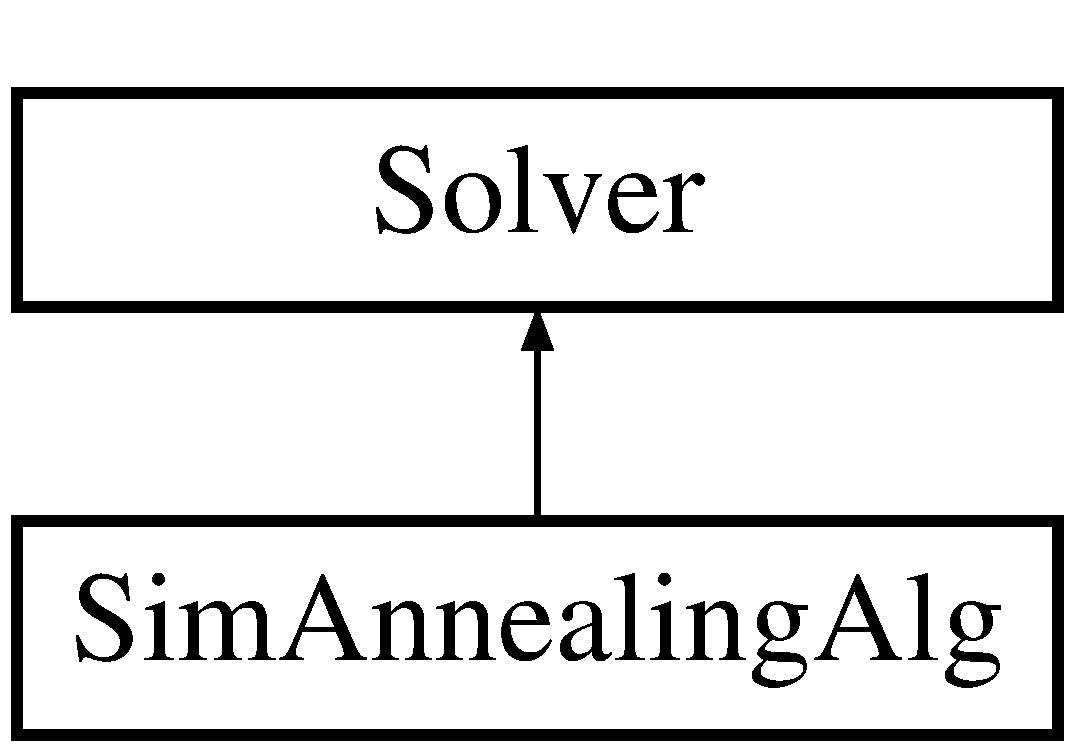
\includegraphics[height=2.000000cm]{classSimAnnealingAlg}
\end{center}
\end{figure}
\subsection*{Static Public Member Functions}
\begin{DoxyCompactItemize}
\item 
virtual static \hyperlink{classRoute}{Route} $\ast$ \hyperlink{classSimAnnealingAlg_adc4279f093215c222928f5a0a2b9c4f0}{solve} (const \hyperlink{classNetwork}{Network} $\ast$n)
\end{DoxyCompactItemize}
\subsection*{Additional Inherited Members}


\subsection{Detailed Description}
Simulated Annealing Algorithm used for finding routes. See doc folder for more information. 

\subsection{Member Function Documentation}
\hypertarget{classSimAnnealingAlg_adc4279f093215c222928f5a0a2b9c4f0}{\index{Sim\+Annealing\+Alg@{Sim\+Annealing\+Alg}!solve@{solve}}
\index{solve@{solve}!Sim\+Annealing\+Alg@{Sim\+Annealing\+Alg}}
\subsubsection[{solve}]{\setlength{\rightskip}{0pt plus 5cm}virtual static {\bf Route}$\ast$ Sim\+Annealing\+Alg\+::solve (
\begin{DoxyParamCaption}
\item[{const {\bf Network} $\ast$}]{n}
\end{DoxyParamCaption}
)\hspace{0.3cm}{\ttfamily [static]}, {\ttfamily [virtual]}}}\label{classSimAnnealingAlg_adc4279f093215c222928f5a0a2b9c4f0}
Method used in \hyperlink{classNetwork}{Network} class for finding best connection between points. 
\begin{DoxyParams}{Parameters}
{\em n} & Pointer to \hyperlink{classNetwork}{Network} in which \hyperlink{classRoute}{Route} is being searched for. \\
\hline
\end{DoxyParams}
\begin{DoxyReturn}{Returns}
Pointer to found \hyperlink{classRoute}{Route}, N\+U\+L\+L if no route can be found. 
\end{DoxyReturn}


Implements \hyperlink{classSolver_ad5eb692895667e7a529bffa5895bf6cc}{Solver}.



The documentation for this class was generated from the following file\+:\begin{DoxyCompactItemize}
\item 
/home/vka/\+Workspace/\+Route\+Finder/src/Sim\+Annealing\+Alg.\+h\end{DoxyCompactItemize}

\hypertarget{classSolver}{\section{Solver Class Reference}
\label{classSolver}\index{Solver@{Solver}}
}


{\ttfamily \#include $<$Solver.\+h$>$}

Inheritance diagram for Solver\+:\begin{figure}[H]
\begin{center}
\leavevmode
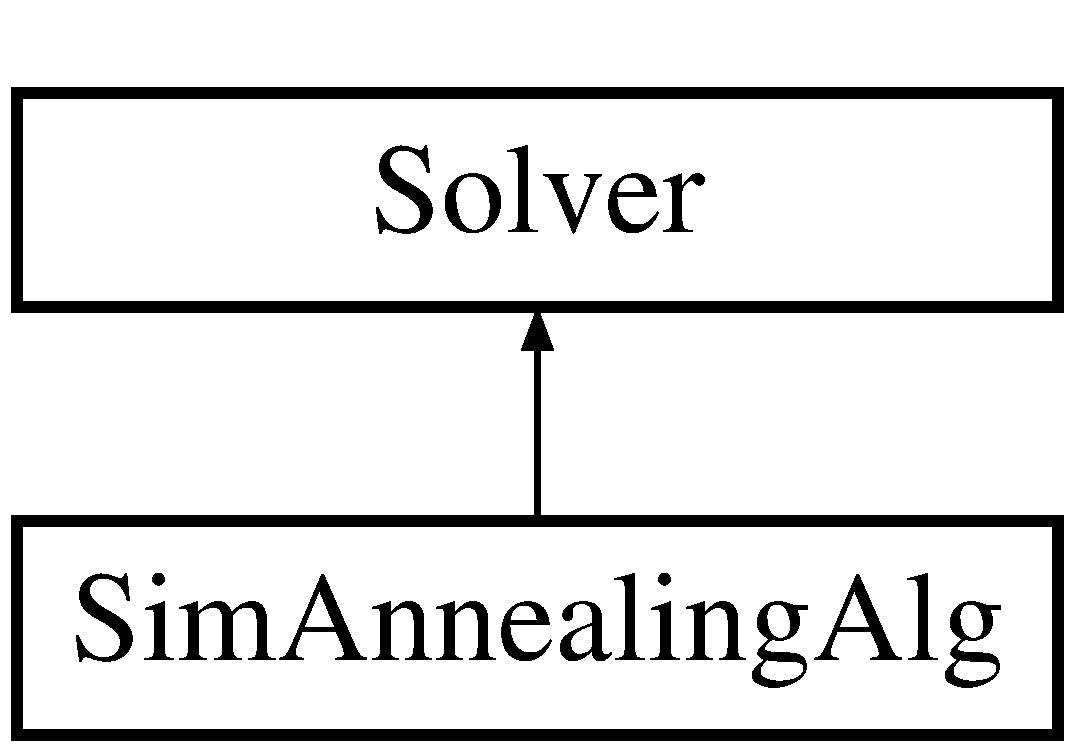
\includegraphics[height=2.000000cm]{classSolver}
\end{center}
\end{figure}
\subsection*{Public Member Functions}
\begin{DoxyCompactItemize}
\item 
virtual \hyperlink{classRoute}{Route} $\ast$ \hyperlink{classSolver_ad5eb692895667e7a529bffa5895bf6cc}{solve} (const \hyperlink{classNetwork}{Network} $\ast$n)=0
\end{DoxyCompactItemize}


\subsection{Detailed Description}
wrapper class for solver algorithm. Those shall inherit from \hyperlink{classSolver}{Solver} class. \hyperlink{classSolver}{Solver} needs to implement solve method, which gets \hyperlink{classNetwork}{Network} map as 

\subsection{Member Function Documentation}
\hypertarget{classSolver_ad5eb692895667e7a529bffa5895bf6cc}{\index{Solver@{Solver}!solve@{solve}}
\index{solve@{solve}!Solver@{Solver}}
\subsubsection[{solve}]{\setlength{\rightskip}{0pt plus 5cm}virtual {\bf Route}$\ast$ Solver\+::solve (
\begin{DoxyParamCaption}
\item[{const {\bf Network} $\ast$}]{n}
\end{DoxyParamCaption}
)\hspace{0.3cm}{\ttfamily [pure virtual]}}}\label{classSolver_ad5eb692895667e7a529bffa5895bf6cc}
Method used in \hyperlink{classNetwork}{Network} class for finding best connection between points. This method need to be implemented in any class inheriting from \hyperlink{classSolver}{Solver} class. 
\begin{DoxyParams}{Parameters}
{\em n} & Pointer to \hyperlink{classNetwork}{Network} in which \hyperlink{classRoute}{Route} is being searched for. \\
\hline
\end{DoxyParams}
\begin{DoxyReturn}{Returns}
Pointer to found \hyperlink{classRoute}{Route}, N\+U\+L\+L if no route can be found. 
\end{DoxyReturn}


Implemented in \hyperlink{classSimAnnealingAlg_adc4279f093215c222928f5a0a2b9c4f0}{Sim\+Annealing\+Alg}.



The documentation for this class was generated from the following file\+:\begin{DoxyCompactItemize}
\item 
/home/vka/\+Workspace/\+Route\+Finder/src/Solver.\+h\end{DoxyCompactItemize}

%--- End generated contents ---

% Index
\newpage
\phantomsection
\addcontentsline{toc}{chapter}{Index}
\printindex

\end{document}
